\documentclass{acm_proc_article-sp}
\usepackage{mdwlist}
\usepackage{xcolor}
\usepackage{enumerate}
\usepackage[colorlinks,
  linkcolor=black,
  anchorcolor=black,
  urlcolor=black,
  citecolor=black
  ]{hyperref}

\begin{document}

\title{An Article Recommendation System\\
Based On Collaborative Topic Modeling}

\numberofauthors{3} 
\author{
\alignauthor
Dang Fan\titlenote{Student ID: 2009013215}\\
       \affaddr{School of Software}\\
       \affaddr{Tsinghua University}\\
       \email{\href{mailto:dangf09@gmail.com}{dangf09@gmail.com}}
\alignauthor
Wang Shuhao\titlenote{Student ID: 2009013229}\\
       \affaddr{School of Software}\\
       \affaddr{Tsinghua University}\\
       \email{\href{mailto:shudiwsh2009@gmail.com}{shudiwsh2009@gmail.com}}
\alignauthor
Ding Peng\titlenote{Student ID: 2009013219}\\
       \affaddr{School of Software}\\
       \affaddr{Tsinghua University}\\
       \email{\href{mailto:dingpeng09@gmail.com}{dingpeng09@gmail.com}}
}

\maketitle
\begin{abstract}
The aim of this report is to describe the algorithm and the implementation of an article recommendation system, which combines the traditional collaborative filtering and probabilistic topic modeling. This system produces latent vectors for both users and articles, which can be used to form recommendations easily. Besides, it can recommend new articles to users without training.
\end{abstract}

% A category with the (minimum) three required fields
\category{H.3.3}{Information Storage and Retrieval}{Information Search and Retrieval}

\terms{Experimentation, Algorithms}

\keywords{recommendation, collaborative filtering, topic modeling} % NOT required for Proceedings

\section{Introduction}
With the rapid development of computers and the Internet, data is becoming unprecedentedly rich, based on which recommendation systems have been focused on for years. According to wikipedia\cite{website:wiki}, three approaches to design a recommendation system are commonly used, which are collaborative filtering, content-based filtering and a hybrid approach.

Collaborative filtering(CF) can be implemented by many different algorithms, for instance, user-based Nearest Neighbor algorithm\cite{website:cf}, and matrix factorization\cite{website:wiki}. However, CF suffers from three problems, cold start, scalability, and sparity.\cite{website:wiki}

Content-based filtering is another common approach. A few algorithms can be used to build a profile of an item (like an article). For example, topic modeling provides a representation of the articles in terms of latent themes discovered from the collection.

In our work, we implement an article recommendation system according to Wang's result\cite{wang:2011:CTM:2020408.2020480}. In this implementation, we combine both the collaborative filtering and the content-based filtering in a probabilistic model.

This paper is organized as follows. In section~\ref{models}, we describe the collaborative topic model we used. In section~\ref{implementation}, we focus on the detail of implementing this system. Section~\ref{performance} contains the evaluation of our implementation and the conclusion (including the limitation).

\section{Collabrotive Topic Modeling}
\label{models}
\subsection{Model}
In this model\cite{wang:2011:CTM:2020408.2020480}, we assume $I$ users and $J$ articles. The rating variable $r_{ij}\in\{0,1\}$ denotes whether user $i$ includes article $j$ in his or her library.

We represent users and articles in the latent topic space of demension $K$ --- user $i$ is represented by a latent vector $u_i \in \mathbb{R}^K$ and article $j$ by a latent vector $v_j \in \mathbb{R}^K$. Then we form the prediction of whether user $i$ will like article $j$ with the inner product between their latent representations,

\begin{equation}\label{eq:prediction}
\hat{r}_{ij}=u_i^Tv_j.
\end{equation}

Then we combine the traditional collabrotive filtering --- matrix factorization\cite{Koren_Bell_Volinsky_2009} and the simplest topic model --- latent Dirichlet allocation (LDA)\cite{Hockenmaier_Blei_Ng_Latent_2009}.

Assume that there are $K$ topics $\beta=\beta_{1:K}$. Then we generate users and articles as follows,

\begin{enumerate}
    \item For each user $i$, draw user latent vector $u_i \sim \mathcal{N}(0,\lambda_u^{-1}I_K)$,

    where $\lambda_u$ is a regularization parameter.
    \item For each article $j$,
       \begin{enumerate}[(a)]
           \item Draw topic distributions $\theta_j \sim$ Dirichlet($\alpha$).
           \item Draw article latent offset $\epsilon_j \sim \mathcal{N}(0, \lambda_v^{-1}I_K)$ and set the article latent vector as $v_j=\epsilon_j+\theta_j$,

           where $\lambda_v$ is a regularization parameter.
           \item For each word $w_{jn}$,
              \begin{enumerate}[i.]
                  \item Draw topic assignment $z_{jn}\sim$ Mult($\theta$).
                  \item Draw word $w_{jw}\sim$ Mult($\beta_{z_{jn}}$).
              \end{enumerate}
       \end{enumerate}
    \item For each user-article pair $(i,j)$, draw the rating
    $$r_{ij}\sim\mathcal{N}(u_i^Tv_j,c_{ij}^{-1}),$$
    where $c_{ij}$ is the precision parameter for $r_{ij}$.
\end{enumerate}

Here, the precision parameter $c_{ij}$ serves as a confidence parameter for rating $r_{ij}$. Thus, we let

\begin{equation*}
  c_{ij}=
  \left\{
   \begin{array}{l}
   a, \text{ if } r_{ij}=1,  \\
   b, \text{ if } r_{ij}=0, \\
   \end{array}
  \right.
\end{equation*}
where $a$ and $b$ are tuning parameters satifying $a>b>0$.

Note that we call this the collaborative topic regression (CTR) model.

\subsection{Learning the parameters}
\label{learning}
In this section, we assume that topic parameter $\beta$ is known after being processed using LDA. Then we focus on how to compute the parameters $u_i, v_j$ and $\theta_j$. According to Wang's result\cite{wang:2011:CTM:2020408.2020480}, an EM-style algorithm can be used to learn the maximum a posteriori estimates.

First, we compute the complete log likelihood of $U, V, \theta_{1:J}$, and $R$ given $\lambda_u, \lambda_v$ and $\beta$,

\begin{equation}
\begin{aligned}
\mathcal{L}&=-\frac{\lambda_u}{2}\Sigma_iu_i^Tu_i-\frac{\lambda_v}{2}\Sigma_j(v_j-\theta_j)^T(v_j-\theta_j)\\
&+\Sigma_j\Sigma_n\log(\Sigma_k\theta_{jk}\beta_{k,w_{jn}})-\Sigma_{i,j}\frac{c_{ij}}{2}(r_{ij}-u_i^Tv_j)^2.\\
\end{aligned}
\end{equation}

To maximize this function, we iteratively optimize the collaborative filtering variables $\{u_i,v_j\}$ and the topic distribution $\theta_j$. In order to do this, we firstly use the following calculation to optimize $u_i, v_j$
\begin{eqnarray}
\begin{aligned}
u_i &\leftarrow (VC_iV^T+\lambda_uI_K)^{-1}VC_iR_i\\
v_j &\leftarrow (UC_jU^T+\lambda_vI_K)^{-1}(UC_jR_j+\lambda_v\theta_j)\\
\end{aligned}
\end{eqnarray}
where $C_i$ is a diagonal matrix with $c_{ij},j=1,\cdots,J$ as its diagonal elements and $R_i=(r_{ij})^J_{j=1}$ for user $i$. For article $j$, $C_j$ and $R_j$ are similarly defined.

As Wang's result\cite{wang:2011:CTM:2020408.2020480} suggests, $\theta_j$ cannot be optimized analytically. In his paper, he uses projection gradient, which is able to be found in his paper.

\section{Implementation}
\label{implementation}
The implementation of this system can be separated into four parts --- preprocessing, LDA processing, CTR processing, and recommending.

\subsection{Preprocessing}
In this stage, we preprocess each article to generate the input file for the sencond stage.

For each article, we concatenate its title and abstract. Using Word Vector Tool\footnote{\url{http://sourceforge.net/projects/wvtool/}}, we remove stop words, stem the rest words, and generate tf-idf vectors. We sum up these vectors and choose the top 8000 words as the vocabulary. After that, we reuse Word Vector Tool to get the term counts vector for each article.

The preprocessor is located at the package \texttt{cn.edu.tsinghua .AR.preprocessor}.

\subsection{LDA Processing}
LDA\cite{Hockenmaier_Blei_Ng_Latent_2009} was first presented by David Blei, Andrew Ng, and Michael Jordan. On Blei's homepage\footnote{\url{http://www.cs.princeton.edu/~blei/}}, a Java-implemented LDA-J project (under GNU GPL v2) from Gregor Heinrich\footnote{\url{http://www.arbylon.net/projects/}} is provided.

We use this package to do LDA processing with some modification required to fit our whole system. The LDA code is located at the package \texttt{org.knowceans.lda} and \texttt{org.knowceans .util}

After this stage, the parameter matrice $\beta$ and $\theta$ are produced.

\subsection{CTR Processing}
The author Wang of this paper, according to which we implement the system, released partial code of this algorithm written in C on his homepage\footnote{\url{http://www.cs.princeton.edu/̃chongw/}}.

The partial CTR code provided by Wang is under GNU GPL v2. It uses GNU Scientific Library to do calculations on matrice and vectors, which is unavailable in Java. Thus we totally reimplement the CTR algorithm in Java based on his C code. We use JAMA\footnote{\url{http://math.nist.gov/javanumerics/jama/}} to do calculations on matrice.

The CTR code is located at the package \texttt{cn.edu.tsinghua.AR .ctr}. It simply follows the learning strategies described in section~\ref{learning}.

After this stage, the latent vectors of users and articles are produced.

\subsection{Recommendation}
As we described in section~\ref{models}, we form the prediction with the inner product between the latent vector of user and article in Eq.~\ref{eq:prediction}.

We compute each prediction in the candidate library for each user, and output the top 5 result as our recommendations.

The code is located at the package \texttt{cn.edu.tsinghua.AR.system}. The program will generate \texttt{result.txt} as the required output file.


\section{Performance and Conclusion}
\label{performance}
\subsection{Evaluation}
To evaluate the result, we use the training data provided by TA as the library. Then we randomly choose at least 5 articles collected by each user as the actual training data, and still choose 250 candidate articles in total.

We evaluate our result with two metrics.

The first metric is accuracy. We compute the average accuracy by

\begin{equation}
\text{Average Accuracy}=\frac{\text{articles in the libarary}}{\text{articles recommended}}
\end{equation}

The second metric is Average Precision at 5(AP@5)\cite{Zhu2004}.

For LDA, we vary $K \in \{25, 50, 75, 100, 125, 150, 175, 200\}$, and set $\alpha=50/K$.

For CTR, we set $a=1, b=0.01, \lambda_u=0.01, \lambda_v=100$, and the same $K$ in LDA.

\subsection{Comparison}

Table~\ref{tab:performance} demonstrates the two metrics we mentioned above and the running time on a 2.4Ghz CPU computer.

\begin{table}[htbp]
\centering
\caption{The performance of AR\label{tab:performance}}
\begin{tabular}{cccc} \hline
$K$ & Accuracy & AP@5 & Running Time\\ \hline
25 & 2.9831 & 0.7435 & 40min\\
50 & 3.4597 & 0.8296 & 54min\\
75 & 3.6293 & 0.8545 & 1.8h\\
100 & 3.7348 & 0.8717 & 3.5h\\
125 & 3.7709 & 0.8794 & 4.3h\\
150 & 3.8080 & 0.8812 & 7.0h\\
175 & 3.8258 & 0.8873 & 9.8h\\
200 & 3.8427 & 0.8881 & 13.2h\\
\hline\end{tabular}
\end{table}

Figure~\ref{fig:acc},\ref{fig:ap} and \ref{fig:time} also show the performance.

\begin{figure}[h]
\begin{minipage}[t]{0.45\linewidth}
\centering
\epsfig{file=acc.eps,width=1.25\textwidth}
\caption{Accuracy\label{fig:acc}}
\end{minipage}
\hfill
\begin{minipage}[t]{0.45\linewidth}
\centering
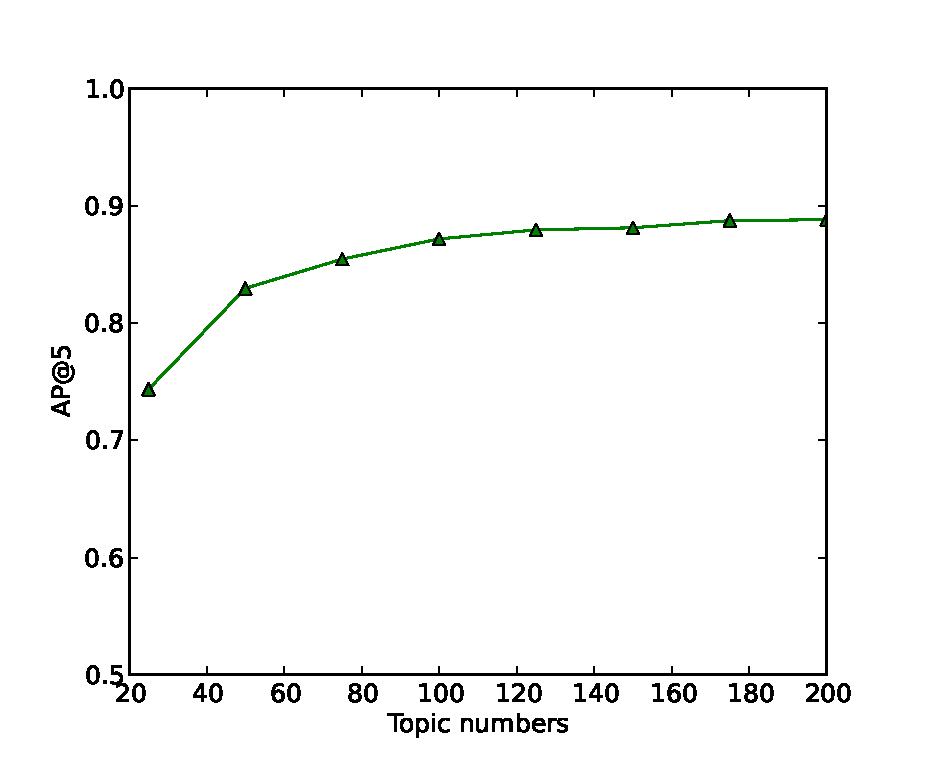
\epsfig{file=ap.eps,width=1.25\textwidth}
\caption{AP@5\label{fig:ap}}
\end{minipage}
\end{figure}

\begin{figure}[htbp]
\centering
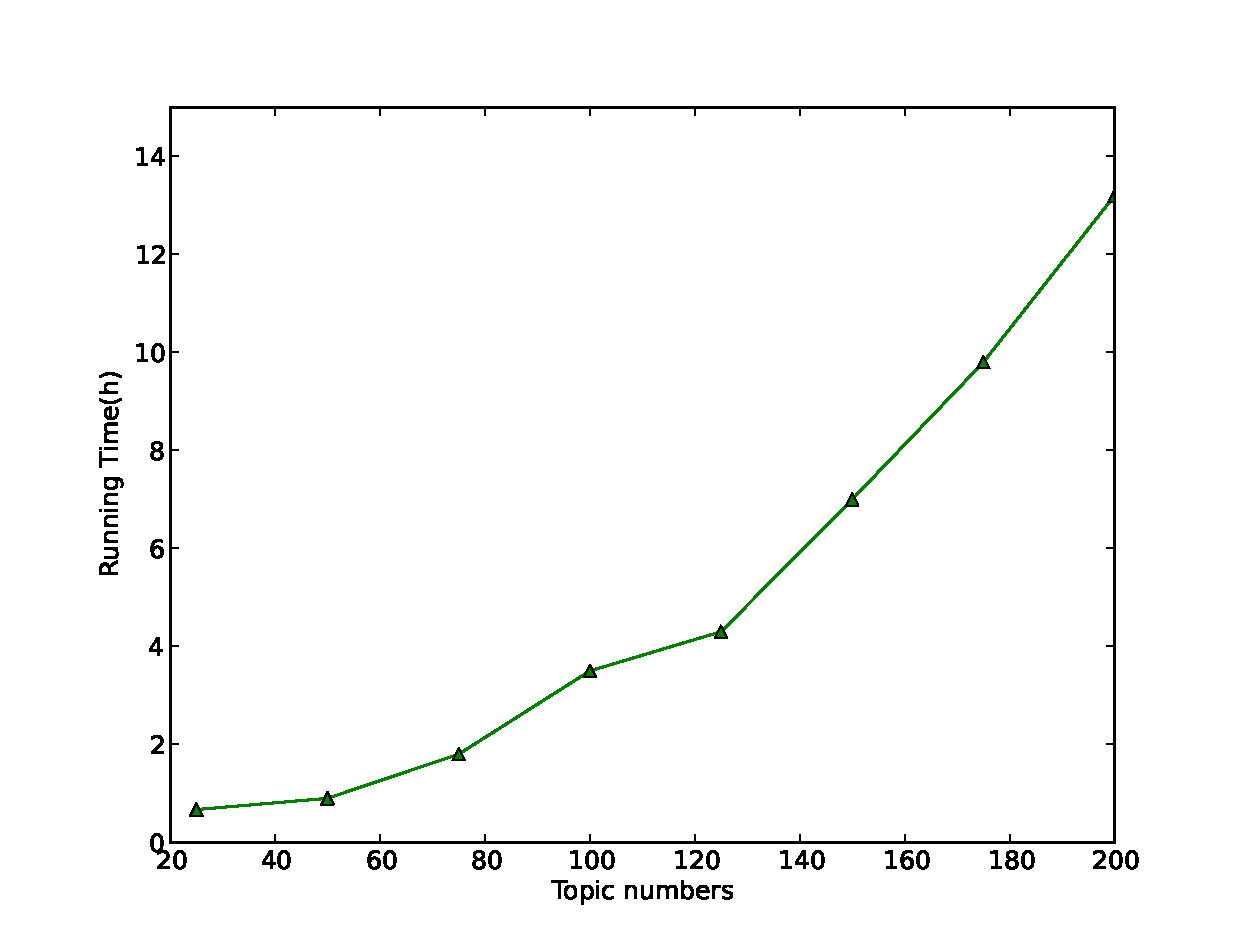
\epsfig{file=time.eps,width=0.3\textwidth}
\caption{AP@5\label{fig:time}}
\end{figure}

From the comparison above, we find that the higher $K$ is, the more precise it is. However, the running time also increases fast. In this case, we think that the result of $K=100$ is fair.

\subsection{Conclusion}
Based on the evaluation, we are able to conclude that the collaborative modeling performs well.

Based on the latent vector and LDA, recommending new articles is also available. LDA can generate inference of a new article, thus we could simply compute the inner product to give a prediction.

However, there are several limitations in this system,
\begin{enumerate}
  \item The running time is very long.
  \item When rating changes, the system has to learn new parameters again.
\end{enumerate}

\section{Acknowledgments}
Thanks to Mr Jin for being such good guider for us. Thanks to TA, Mr Ding, for answering our questions.

%
% The following two commands are all you need in the
% initial runs of your .tex file to
% produce the bibliography for the citations in your paper.
\bibliographystyle{plain}
\bibliography{sigproc}

\balancecolumns
% That's all folks!
\end{document}
